%%%%%%%%%%%%%%%%%%%%%%%%%%%%%%%%%%%%%%%%%
% University/School Laboratory Report
% LaTeX Template
% Version 3.0 (4/2/13)
%
% This template has been downloaded from:
% http://www.LaTeXTemplates.com
%
% Original author:
% Linux and Unix Users Group at Virginia Tech Wiki 
% (https://vtluug.org/wiki/Example_LaTeX_chem_lab_report)
%
% License:
% CC BY-NC-SA 3.0 (http://creativecommons.org/licenses/by-nc-sa/3.0/)
%
%%%%%%%%%%%%%%%%%%%%%%%%%%%%%%%%%%%%%%%%%

%----------------------------------------------------------------------------------------
%	PACKAGES AND DOCUMENT CONFIGURATIONS
%----------------------------------------------------------------------------------------

\documentclass{article}

\usepackage{mhchem} % Package for chemical equation typesetting
\usepackage{siunitx} % Provides the \SI{}{} command for typesetting SI units
\usepackage{listings}
\usepackage{commath}
\usepackage{graphicx} % Required for the inclusion of images
\usepackage[margin=1in]{geometry}
\usepackage{multirow}
\usepackage{array}
\setlength\parindent{0pt} % Removes all indentation from paragraphs


%\usepackage{times} % Uncomment to use the Times New Roman font

%----------------------------------------------------------------------------------------
%	DOCUMENT INFORMATION
%----------------------------------------------------------------------------------------

\title{ Homework 1 \\ COSC 594} % Title

\author{Jiahui \textsc{Guo}} % Author name

\date{Jan. 22, 2014} % Date for the report

\begin{document}

\maketitle % Insert the title, author and date

% If you wish to include an abstract, uncomment the lines below
% \begin{abstract}
% Abstract text
% \end{abstract}

%----------------------------------------------------------------------------------------
%	SECTION 1
%----------------------------------------------------------------------------------------

\section{Program Implementation}

\subsection{Test Data}
The vector and matrix are initialized with random number ranging from 0 to 100. 
\subsection{Result verification}
To verify the correctness of the program, I use CBLAS library to compute an accurate result, 
and then calculate the error between the accurate result and computed result, and the error is
measured in 2-norm. The criterion to state a result is accurate needs to meet
\begin{equation*}
    \norm{(accurate-computed)}\le10^{-16}
\end{equation*}

\subsection{Time Measurement}
C timer is used to measure the execution time of each executable. Data generation, memory allocation
and deallocation, and initialization are not included in the execution time, so as to flops.

\subsection{Organization of the program}
The program is organized in the following way:
\begin{description}
    \item[src]/
        \begin{description}
            \item[twoNorm.c] 2-norm of vector
            \item[vecMul.c] Vector-matrix multiplication
            \item[matMul.c] Matrix-matrix multiplication
            \item[c\_timer.c]
            \item[Makefile] 
        \end{description}
    \item[include]/
        \begin{description}
            \item[c\_timer.h]
            \item[cblas.h] 
        \end{description}
    \item[bin]/
        \begin{description}
            \item[run.sh] Run the executable files and generates plots
            \item[avg.py] Average the time and flops obtained from several trials
            \item[plotTime.gnu]
            \item[plotFlops.gnu]
            \item[plotAvgTime.gnu]
            \item[plotAvgFlops.gnu]
        \end{description}
    \item[pdf]/
        \begin{description}
            \item[hw1.tex]
            \item[Makefile]
        \end{description}
    \item[Makefile]
    \item[ReadMe] Illustrating how to execute the program.
\end{description}

\newpage
\section{Experiment Platform}
The experiment was conducted on a hydra machine. The configuration of the machine is list below:
\begin{description}
\item[Processor] Intel Core i7-3770 $@$ 3.40GHz
\item[Memory] 16.0GB DDR3
\item[Hard drive] 500GB 7200 RPM SATA $@$ 6Gbps, 16MB cache
\end{description}

\newpage
\section{Performance Analysis}

\subsection{Operation Analysis}
\begin{enumerate}
\item 2-norm of vector\\
    The operations for 2-norm of a size $N$ vector are $2N$, there is also one multiplication and one
    addition for each data.
\item Vector-matrix multiplication\\
    The operations for vector-matrix multiplication is $2N^2$,  there is also $\theta(N)$ multiplication
    and $\theta(N)$ addition for $N$ element in the result vector.
\item Matrix-matrix multiplication\\
    The Operations for matrix-matrix multiplication is $2N^3$,  there is also $\theta(N)$ multiplication
    and $\theta(N)$ addition for $N$ element in the result matrix.
\end{enumerate}

\subsection{Theoratical Peak Performance}
For the machine used in the experiment, the peak flop per second for one core is calculated as:\\
\begin{equation*}
4\:flops/cycle\:*\:3.40\:G\:cycles\:=\:13.6\:Gflops 
\end{equation*}

\subsection{Experiment Results}
    \begin{figure}[th!]
        \centering
        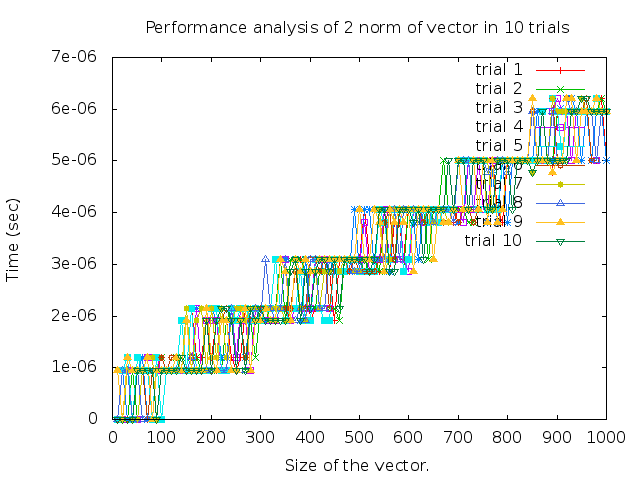
\includegraphics[width=0.8\textwidth]{timingTwoNorm.png}
        \label{fig:timeTwoNorm}
        \caption{Execution time of 2-norm of vector in 10 trials}
    \end{figure}

    \begin{figure}[th!]
        \centering
        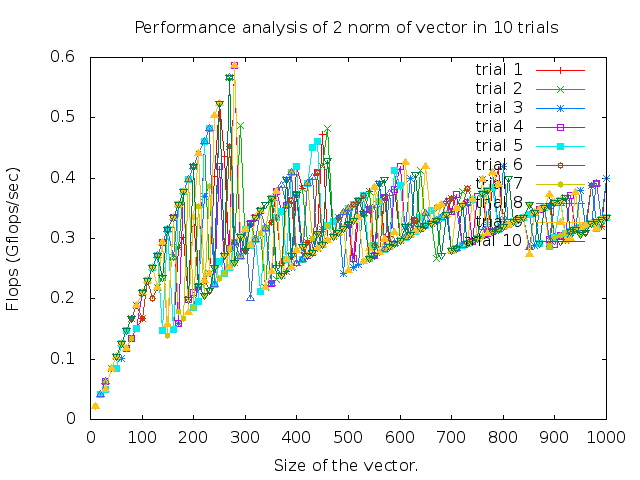
\includegraphics[width=0.8\textwidth]{flopsTwoNorm.png}
        \label{fig:flopsTwoNorm}
        \caption{Flops of 2-norm of vector in 10 trials}
    \end{figure}
    
    \begin{figure}[th!]
        \centering
        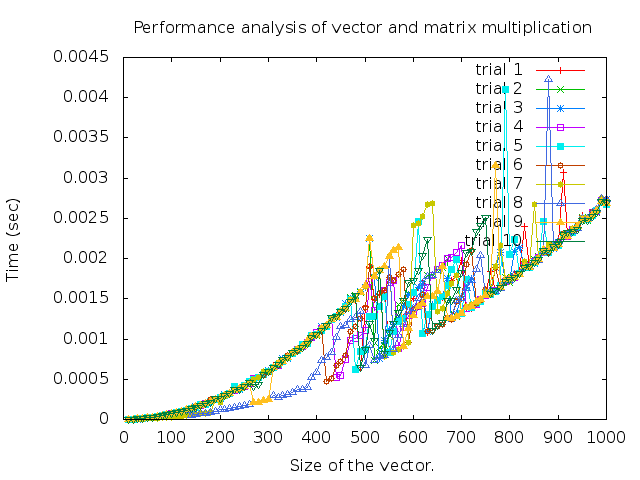
\includegraphics[width=0.8\textwidth]{timingVecMul.png}
        \label{fig:timeVecMul}
        \caption{Execution time of vector-matrix multiplication in 10 trials}
    \end{figure}
    \begin{figure}[th!]
        \centering
        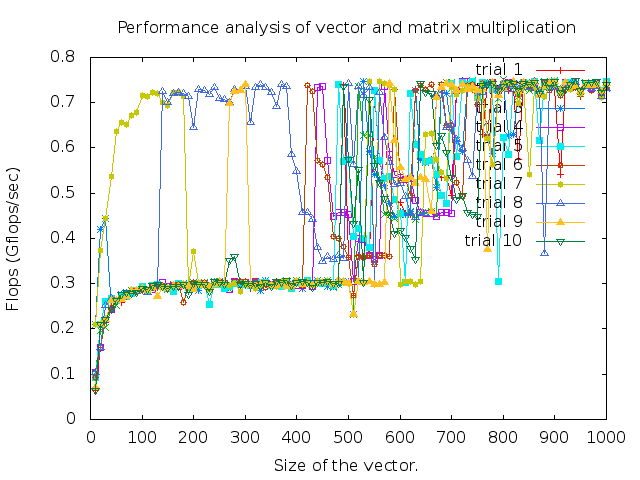
\includegraphics[width=0.8\textwidth]{flopsVecMul.png}
        \label{fig:flopsVecMul}
        \caption{Flops of vector-matrix multiplication in 10 trials}
    \end{figure}

    \begin{figure}[th!]
        \centering
        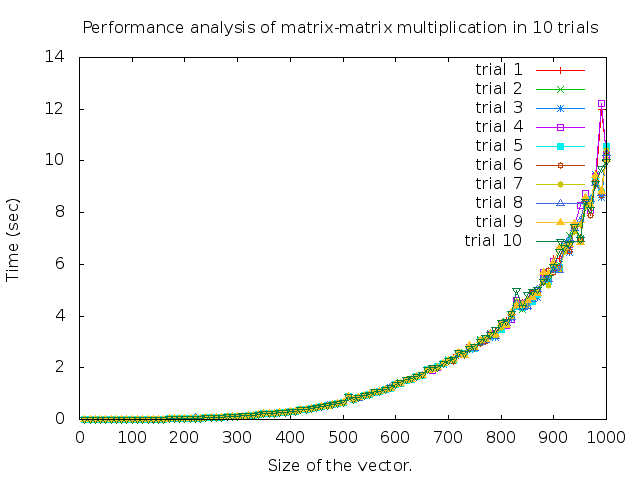
\includegraphics[width=0.8\textwidth]{timingMatMul.png}
        \label{fig:timeMatMul}
        \caption{Execution time of matrix-matrix multiplication in 10 trials}
    \end{figure}

    \begin{figure}[th!]
        \centering
        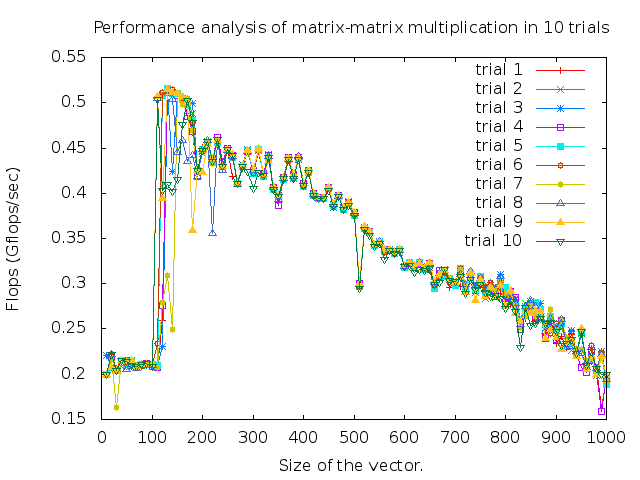
\includegraphics[width=0.8\textwidth]{flopsMatMul.png}
        \label{fig:flopsMatMul}
        \caption{Flops of matrix-matrix multiplication in 10 trials}
    \end{figure}

    \begin{figure}[th!]
        \centering
        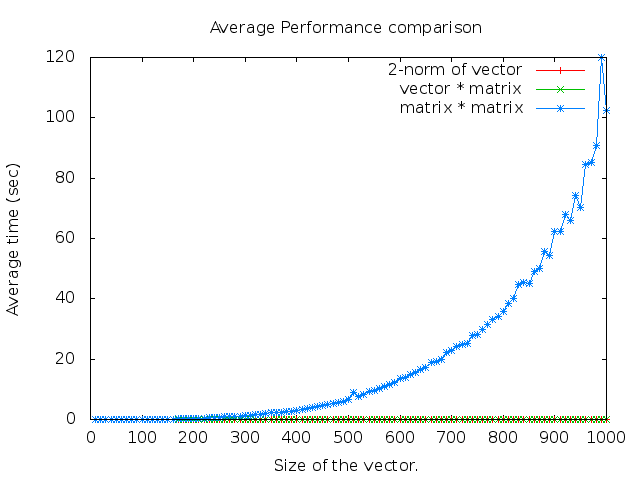
\includegraphics[width=0.8\textwidth]{timingAvg.png}
        \label{fig:timeAvg}
        \caption{Comparison of execution time}
    \end{figure}

    \begin{figure}[th!]
        \centering
        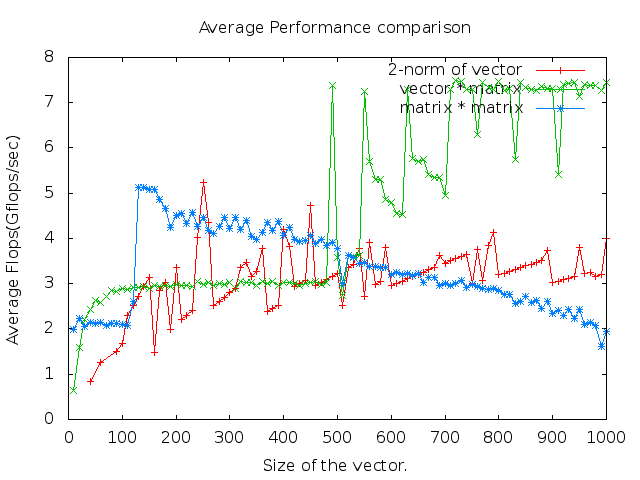
\includegraphics[width=0.8\textwidth]{flopsAvg.png}
        \label{fig:flopsAvg}
        \caption{Comparison of flops}
    \end{figure}

\begin{enumerate}
\item 2-norm of vector
    In Fig.1 and Fig.2, the execution time and flops of 2-norm of vector computation is shown. The peak Gops/sec is around 0.6 GFlops. Execution time keeps increasing with larger input data size.

\item Vector-matrix multiplication
   In Fig.3 and Fig.4, the execution time and flops of vector-matrix multiplication computation is shown. The peak Gops/sec is around 0.75 GFlops. Execution time keeps increasing with larger input data size exponentially.

\item Matrix-matrix multiplication
   In Fig.5 and Fig.6, the execution time and flops of matrix-matrix multiplication computation is shown. The peak Gops/sec is around 0. 5 GFlops. Execution time keeps increasing with larger input data size exponentially.

\item Average execution time and flops comparison
   In Fig.7 and Fig.8, the execution time and flops of these three programs are compared.
   It can be seen that with the increasing of input data size, matrix-matrix multiplication will consuming much more
   time than the other two, and the execution time is incresing exponentially. Also, one thing needs to be addressed is
   that the flops for matrix-matrix multiplication would get worse with the increasing of input data size because of the memory issue.
\end{enumerate}



\newpage
\subsection{Discuss}
\begin{enumerate}
\item Why the achieved performance is different than the peak?
    \begin{enumerate}
        \item Program implementation is not efficient enough;
        \item System resources are occupied by other programs at the same time;
    \end{enumerate}
\item How to improve the performance?
    \begin{enumerate}
        \item Increasing core frequency level;
        \item Improving instruction level;
        \item Optimizing the program;
        \item Multithreading or parallel;
        \item Larger cache.
    \end{enumerate}
\end{enumerate}

\end{document}
